\documentclass[a4paper,utf8]{article}
\usepackage[heading,fancyhdr]{ctex}
\usepackage{amsmath,amssymb,geometry,lastpage,ulem}
\usepackage{array,tabularx,tabulary,mhchem,xspace}
\usepackage{floatrow,subfig,multirow,bigstrut}
\usepackage{siunitx,booktabs,longtable,graphicx,xfrac,nameref}
\lineskiplimit=1pt
\lineskip=3pt
\geometry{
    top=25.4mm, 
    left=25mm, 
    right=25mm, 
    bottom=25mm,
    headsep=5.9mm,
}
\ctexset{
    section = {format+=\raggedright}
}
\newcommand{\fgref}[1]{图~\ref{#1}\xspace}
\newcommand{\seqref}[1]{式~(\ref{#1})}
\newcommand{\expinfo}[7][无]{
    {\zihao{-3}\bfseries\songti
    实验名称:\uline{\hfill\mbox{#2}\hfill} \\[2.9mm]
    学\quad 号:\uline{\makebox[25mm]{#3}}\hfill
    姓\quad 名:\uline{\makebox[25mm]{#4}}\hfill
    班\quad 级:\uline{\makebox[25mm]{#5}} \\[2.9mm]
    合作者:\uline{\makebox[25mm]{#1}} \hfill
    桌\quad 号:\uline{\makebox[25mm]{#6}}\hfill\makebox[25mm+4em]{}\\[2.9mm]
    实验日期:\uline{\makebox[30mm]{#7}}\hfill\mbox{} \\[58.7mm]
    }
}
\newcommand{\pointingbox}{
    {\zihao{4}\bfseries\songti%
    实验考核\\[3mm]
    \extrarowheight=3mm
    \begin{tabularx}{150mm}{|X|X|X|X|X|}\hline
        \hfil 项目 \hfil  & \hfil 实验预习 \hfil & \hfil 实验过程 \hfil & \hfil 分析与讨论 \hfil & \hfil 总评 \hfil \\[3mm] \hline
        \hfil 评价 \hfil &  &  &  &  \\[3mm] \hline
    \end{tabularx}
    }
}
\newcommand{\derivative}[2]{\frac{\mathrm{d} #1}{\mathrm{d} #2}}
\newcommand{\thinking}[2]{\textbf{#1}\\
答:\begin{minipage}[t]{0.85\textwidth}
    #2
\end{minipage}}
\pagestyle{fancy}
\fancyhf{} \fancyhead[C]{电路基础实验} \fancyfoot[C]{\thepage~/~\pageref{LastPage}}
\newcounter{Rownumber}
\newcommand*{\Rown}{\stepcounter{Rownumber}\theRownumber}
\newcommand*{\resetRown}{\setcounter{Rownumber}{0}}
\newcommand{\qrange}[3]{\qtyrange[range-phrase = \text{$\sim$},range-units =single]{#1}{#2}{#3}}
\floatsetup[table]{capposition=top}
\newcolumntype{C}{>{\hfil}X<{\hfil}}
\renewcommand{\Nameref}[1]{\textbf{\ref{#1}~\nameref{#1}}} %导入导言
\ExecuteOptions{draft}
\begin{document}
\begin{center}
    {\mbox{}\\[7em]\zihao{2}\bfseries\songti%
    电路基础实验报告}\\[34mm]
    \expinfo[王慷]{R、L、C 元件阻抗特性的研究}{22301056}{王俊杰}{22 材物}{27}{2024.6.18}
\end{center}
\newpage

\section{实验目的}
\begin{enumerate}
    \item 验证电阻、感抗、容抗与频率的关系,测定 $R-f$、$X_\text{L}-f$ 及 $X_\text{C}-f$ 特性曲线。
    \item 加深理解 R、L、C 元件端电压与电流间的相位关系。
\end{enumerate}

\section{实验原理}%简单描述,含必要的公式和附图;
在正弦交变信号作用下,$R$、$L$、$C$ 电路元件在电路中的抗流作用与信号的频率有关。\par
改变信号源频率,测量 $R$、$L$、$C$ 元件两端电压 $U_\text{R}$、$U_\text{L}$、$U_\text{C}$,流过被测元件的电流则可由 $r$ 两端电压除以 $r$ 得到。\par
元件的阻抗角(即相位差 $\varphi$)随输入信号的频率变化而改变,将各个不同频率下的相位差画在以频率 f 为横坐标、阻抗角 $\varphi$ 为纵座标的座标纸上,并用光滑的曲线连接这些点,即得到阻抗角的频率特性曲线。 

\section{实验仪表}
    实验电路见电路原理实验箱《二阶电路动态过程的研究》单元,$L=\SI{10}{\mH}$,$r=\SI{200}{\ohm}$,$C=\SI{1}{\uF}$。

\section{实验内容}
\begin{enumerate}
    \item 测量 $R$、$L$、$C$ 元件的阻抗频率特性。
    \item 用双踪示波器观察 RL 串联和 RC 串联电路在不同频率下阻抗角的变化情况。
\end{enumerate}
\section{实验结果与分析}
\subsection{实验数据}
\begin{longtable}{
    S[table-format=6.2] S[table-format=3.5] S[table-format=3.6]%
    S[table-format=3.5] S[table-format=6.3]}

    \caption{电阻阻抗频率特性测量结果\label{tab:11.Rvsf}} \\ \toprule
    {$f$(\unit{\Hz})} & {$U_\text{R}$(\unit{\V})} & {$U_\text{r}$(\unit{\V})} & {$I_\text{r}$(\unit{\mA})} & {$R$(\unit{\ohm})} \\ \midrule
    \endfirsthead
    \multicolumn{5}{r}{\small 表 \ref{tab:11.Rvsf} (续)} \\ \toprule
    {$f$(\unit{\Hz})} & {$U_\text{R}$(\unit{\V})} & {$U_\text{r}$(\unit{\V})} & {$I_\text{r}$(\unit{\mA})} & {$R$(\unit{\ohm})} \\ \midrule
    \endhead

    \bottomrule
    \endfoot

    \bottomrule
    \endlastfoot

    200 & 2.505 & 0.4970 & 2.485 & 1008.0 \\ 
    500 & 2.438 & 0.4860 & 2.430 & 1003.3 \\ 
    800 & 2.458 & 0.4900 & 2.450 & 1003.3 \\ 
    1100 & 2.459 & 0.4910 & 2.455 & 1001.6 \\ 
    1400 & 2.454 & 0.4900 & 2.450 & 1001.6 \\ 
    1700 & 2.443 & 0.4900 & 2.450 & 997.1 \\ 
    2000 & 2.454 & 0.4910 & 2.455 & 999.6 \\ 
    2300 & 2.422 & 0.4850 & 2.425 & 998.8 \\ 
    2600 & 2.409 & 0.4827 & 2.414 & 998.1 \\ 
    2900 & 2.414 & 0.4849 & 2.425 & 995.7 \\ 
    3200 & 2.426 & 0.4868 & 2.434 & 996.7 \\ 
    3500 & 2.454 & 0.4923 & 2.462 & 997.0 \\ 
    3800 & 2.400 & 0.4812 & 2.406 & 997.5 \\ 
    4100 & 2.469 & 0.4943 & 2.472 & 999.0 \\ 
    4400 & 2.407 & 0.4824 & 2.412 & 997.9 \\ 
    4700 & 2.447 & 0.4903 & 2.452 & 998.2 \\ 
    5000 & 2.432 & 0.4878 & 2.439 & 997.1 \\ 
\end{longtable}

\begin{longtable}{
    S[table-format=6.2] S[table-format=3.5] S[table-format=3.6]%
    S[table-format=3.5] S[table-format=5.3] S[table-format=3.1]%
    S[table-format=3.1] S[table-format=4.3]}

    \caption{电感阻抗频率特性测量结果\label{tab:11.Lvsf}} \\ \toprule
    {$f$(\unit{\Hz})} & {$U_\text{R}$(\unit{\V})} & {$U_\text{r}$(\unit{\V})} & {$I_\text{r}$(\unit{\mA})} & {$\left|Z\right|$(\unit{\ohm})} & {$m$} & {$n$} & {$\varphi$(${}^\circ$)}\\ \midrule
    \endfirsthead
    \multicolumn{8}{r}{\small 表 \ref{tab:11.Lvsf} (续)} \\ \toprule
    {$f$(\unit{\Hz})} & {$U_\text{R}$(\unit{\V})} & {$U_\text{r}$(\unit{\V})} & {$I_\text{r}$(\unit{\mA})} & {$\left|Z\right|$(\unit{\ohm})} & {$m$} & {$n$} & {$\varphi$(${}^\circ$)} \\ \midrule
    \endhead

    \bottomrule
    \endfoot

    \bottomrule
    \endlastfoot

    200 & 0.601 & 1.9380 & 9.690 & 62.0 & 3 & 50 & 21.6 \\ 
    500 & 0.676 & 1.9330 & 9.665 & 69.9 & 5 & 50 & 36.0 \\ 
    800 & 0.777 & 1.9330 & 9.665 & 80.4 & 4 & 31 & 46.5 \\ 
    1100 & 0.903 & 1.9060 & 9.530 & 94.8 & 6 & 45 & 48.0 \\ 
    1400 & 1.019 & 1.8440 & 9.220 & 110.5 & 5 & 36 & 50.0 \\ 
    1700 & 1.171 & 1.8130 & 9.065 & 129.2 & 10 & 59 & 61.0 \\ 
    2000 & 1.315 & 1.7420 & 8.710 & 151.0 & 9 & 50 & 64.8 \\ 
    2300 & 1.439 & 1.7130 & 8.565 & 168.0 & 8 & 43 & 67.0 \\ 
    2600 & 1.543 & 1.6720 & 8.360 & 184.6 & 7 & 38 & 66.3 \\ 
    2900 & 1.639 & 1.6480 & 8.240 & 198.9 & 7 & 34 & 74.1 \\ 
    3200 & 1.733 & 1.6040 & 8.020 & 216.1 & 6 & 31 & 69.7 \\ 
    3500 & 1.807 & 1.5760 & 7.880 & 229.3 & 6 & 28 & 77.1 \\ 
    3800 & 1.861 & 1.5400 & 7.700 & 241.7 & 5 & 26 & 69.2 \\ 
    4100 & 1.975 & 1.4920 & 7.460 & 264.7 & 12 & 61 & 70.8 \\ 
    4400 & 2.072 & 1.4130 & 7.065 & 293.3 & 12 & 57 & 75.8 \\ 
    4700 & 2.100 & 1.3900 & 6.950 & 302.2 & 11 & 53 & 74.7 \\ 
    5000 & 2.173 & 1.3500 & 6.750 & 321.9 & 11 & 50 & 79.2 \\ 
\end{longtable}

\begin{longtable}{
    S[table-format=6.2] S[table-format=3.5] S[table-format=3.6]%
    S[table-format=3.5] S[table-format=5.3] S[table-format=3.1]%
    S[table-format=3.1] S[table-format=4.3]}

    \caption{电容阻抗频率特性测量结果\label{tab:11.Cvsf}} \\ \toprule
    {$f$(\unit{\Hz})} & {$U_\text{R}$(\unit{\V})} & {$U_\text{r}$(\unit{\V})} & {$I_\text{r}$(\unit{\mA})} & {$\left|Z\right|$(\unit{\ohm})} & {$m$} & {$n$} & {$\varphi$(${}^\circ$)}\\ \midrule
    \endfirsthead
    \multicolumn{8}{r}{\small 表 \ref{tab:11.Cvsf} (续)} \\ \toprule
    {$f$(\unit{\Hz})} & {$U_\text{R}$(\unit{\V})} & {$U_\text{r}$(\unit{\V})} & {$I_\text{r}$(\unit{\mA})} & {$\left|Z\right|$(\unit{\ohm})} & {$m$} & {$n$} & {$\varphi$(${}^\circ$)} \\ \midrule
    \endhead

    \bottomrule
    \endfoot

    \bottomrule
    \endlastfoot

    200 & 2.946 & 0.714 & 3.571 & 825.0 & -6 & 25 & -86.4 \\ 
    340 & 2.638 & 1.150 & 5.750 & 458.8 & -7 & 29.5 & -85.4 \\ 
    480 & 2.437 & 1.450 & 7.250 & 336.1 & -5.5 & 21 & -94.3 \\ 
    620 & 2.170 & 1.679 & 8.395 & 258.5 & -10.5 & 40.5 & -93.3 \\ 
    760 & 1.926 & 1.870 & 9.350 & 206.0 & -8.5 & 33 & -92.7 \\ 
    900 & 1.753 & 1.964 & 9.820 & 178.5 & -7 & 28 & -90.0 \\ 
    1040 & 1.566 & 2.080 & 10.400 & 150.6 & -6 & 24 & -90.0 \\ 
    1180 & 1.426 & 2.139 & 10.695 & 133.3 & -10 & 42 & -85.7 \\ 
    1320 & 1.346 & 2.141 & 10.705 & 125.7 & -9 & 38 & -85.3 \\ 
    1460 & 1.227 & 2.194 & 10.970 & 111.9 & -8 & 34 & -84.7 \\ 
    1600 & 1.131 & 2.227 & 11.135 & 101.6 & -7.5 & 31.5 & -85.7 \\ 
    1740 & 1.053 & 2.260 & 11.300 & 93.2 & -7 & 29 & -86.9 \\ 
    1880 & 1.003 & 2.251 & 11.255 & 89.1 & -7 & 26.5 & -95.1 \\ 
    2020 & 0.934 & 2.277 & 11.385 & 82.0 & -6 & 25 & -86.4 \\ 
    2160 & 0.871 & 2.307 & 11.535 & 75.5 & -6 & 23 & -93.9 \\ 
    2300 & 0.821 & 2.323 & 11.615 & 70.7 & -11 & 43.5 & -91.0 \\ 
    2440 & 0.786 & 2.352 & 11.760 & 66.8 & -11 & 41 & -96.6 \\ 
\end{longtable}
\subsection{数据处理}
将测量的数据进行分析,并利用公式
\begin{align*}
    \left|Z\right|&=\sqrt{R^2+X^2} & X_\text{L} &=\omega L= 2\pi f L\\
    \varphi&=\arctan\left(\frac X R\right) & X_\text{C} &= \frac{1}{\omega C}=\frac{1}{2\pi f C}
\end{align*}
可以得到所测数据的拟合曲线,如图~\ref{fig:11.inductor}、图~\ref{fig:11.capacitor} 所示。
\begin{figure}[!ht]
    \caption{电感阻抗-频率特性曲线\label{fig:11.inductor}}
    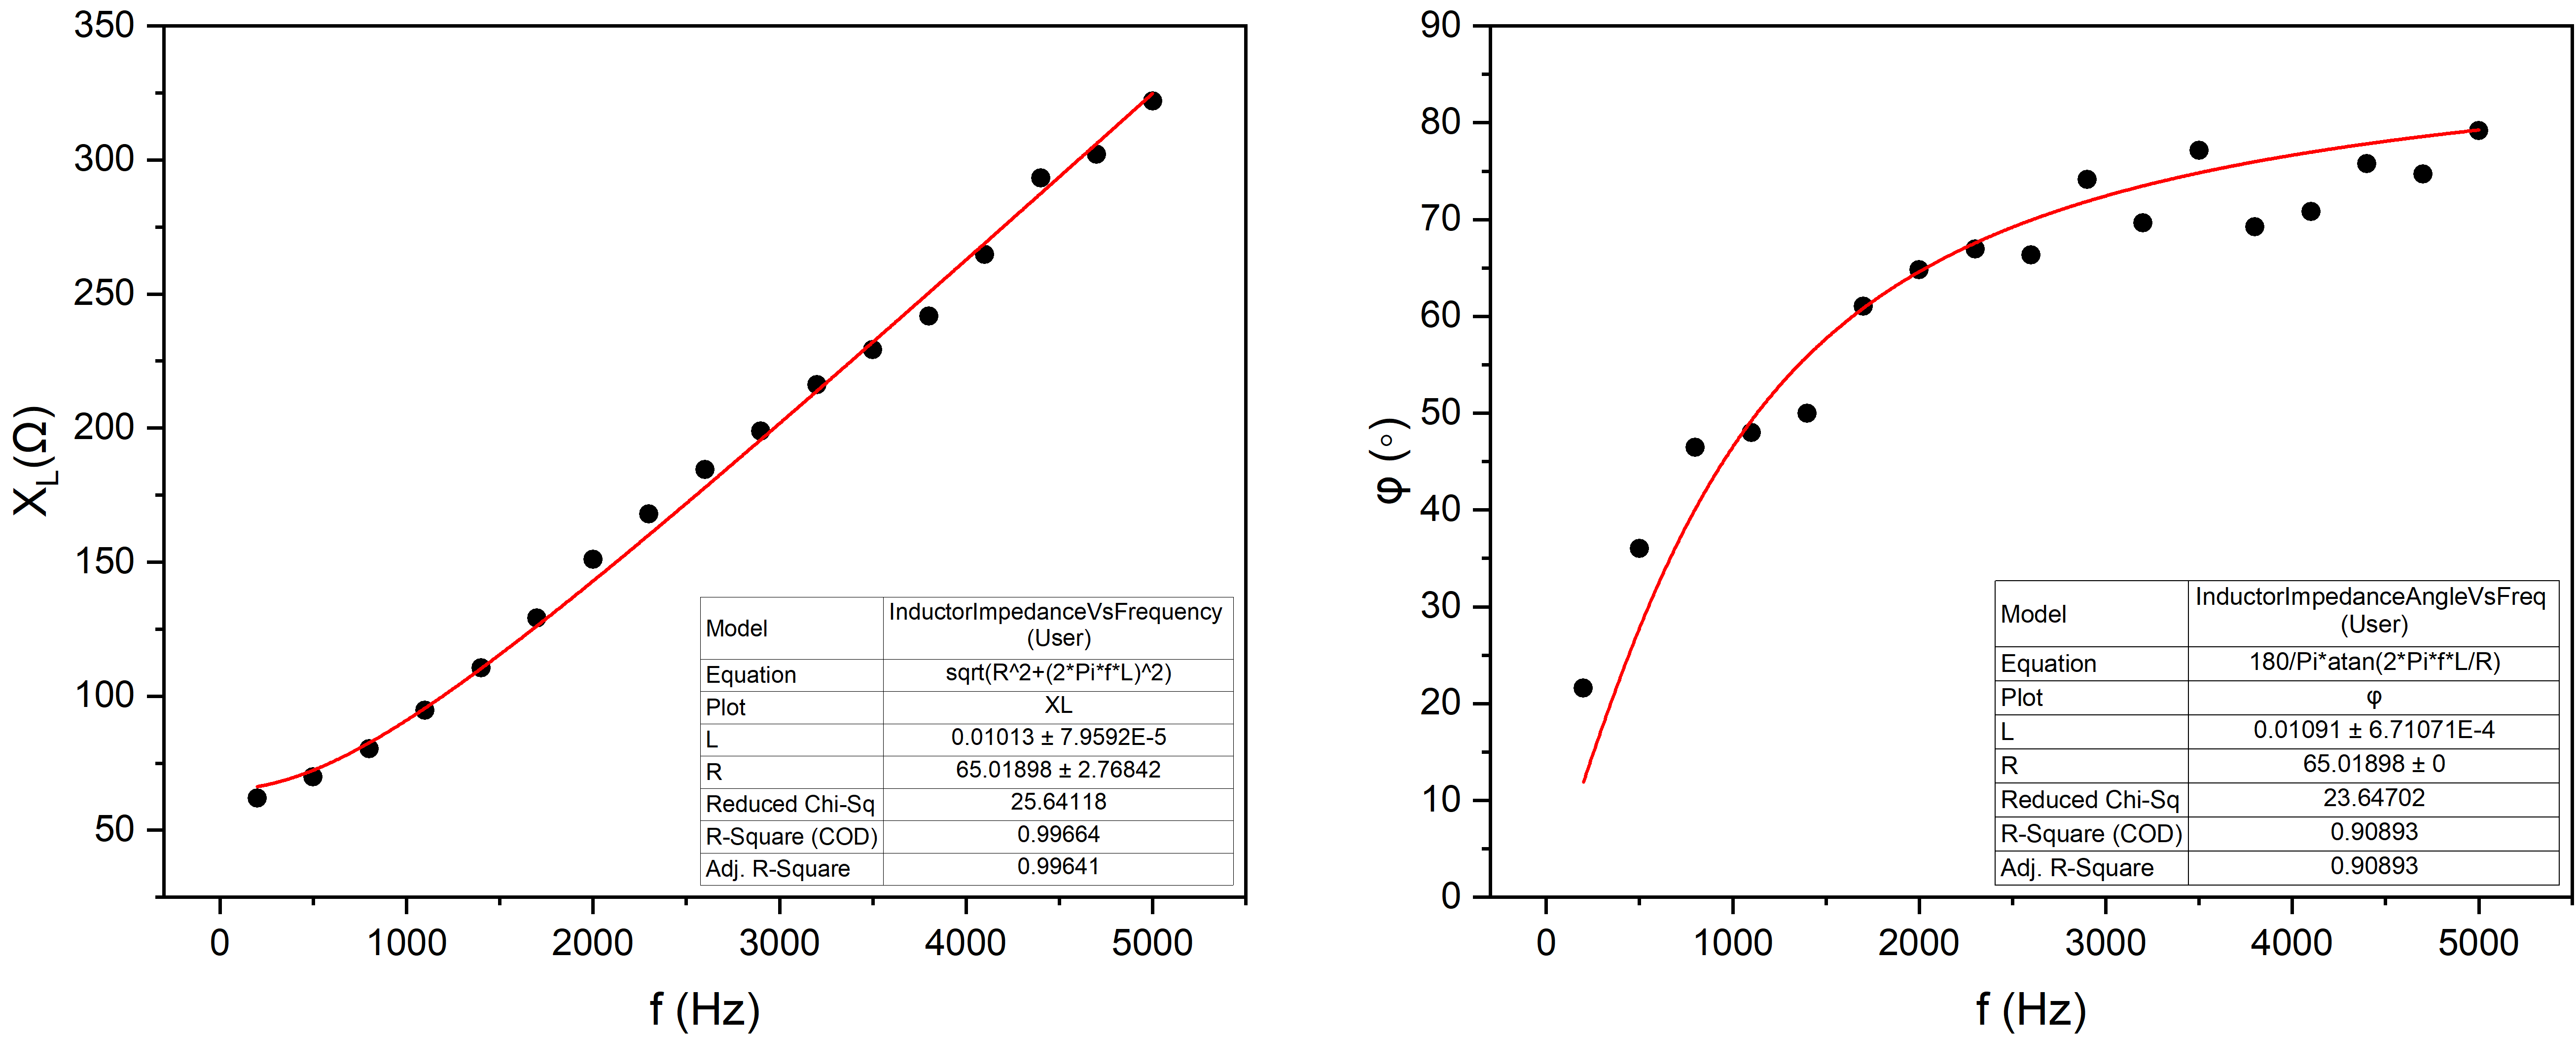
\includegraphics[width=0.9\textwidth]{Inductor.png}
\end{figure}
\begin{figure}[!ht]
    \caption{电容阻抗-频率特性曲线\label{fig:11.capacitor}}
    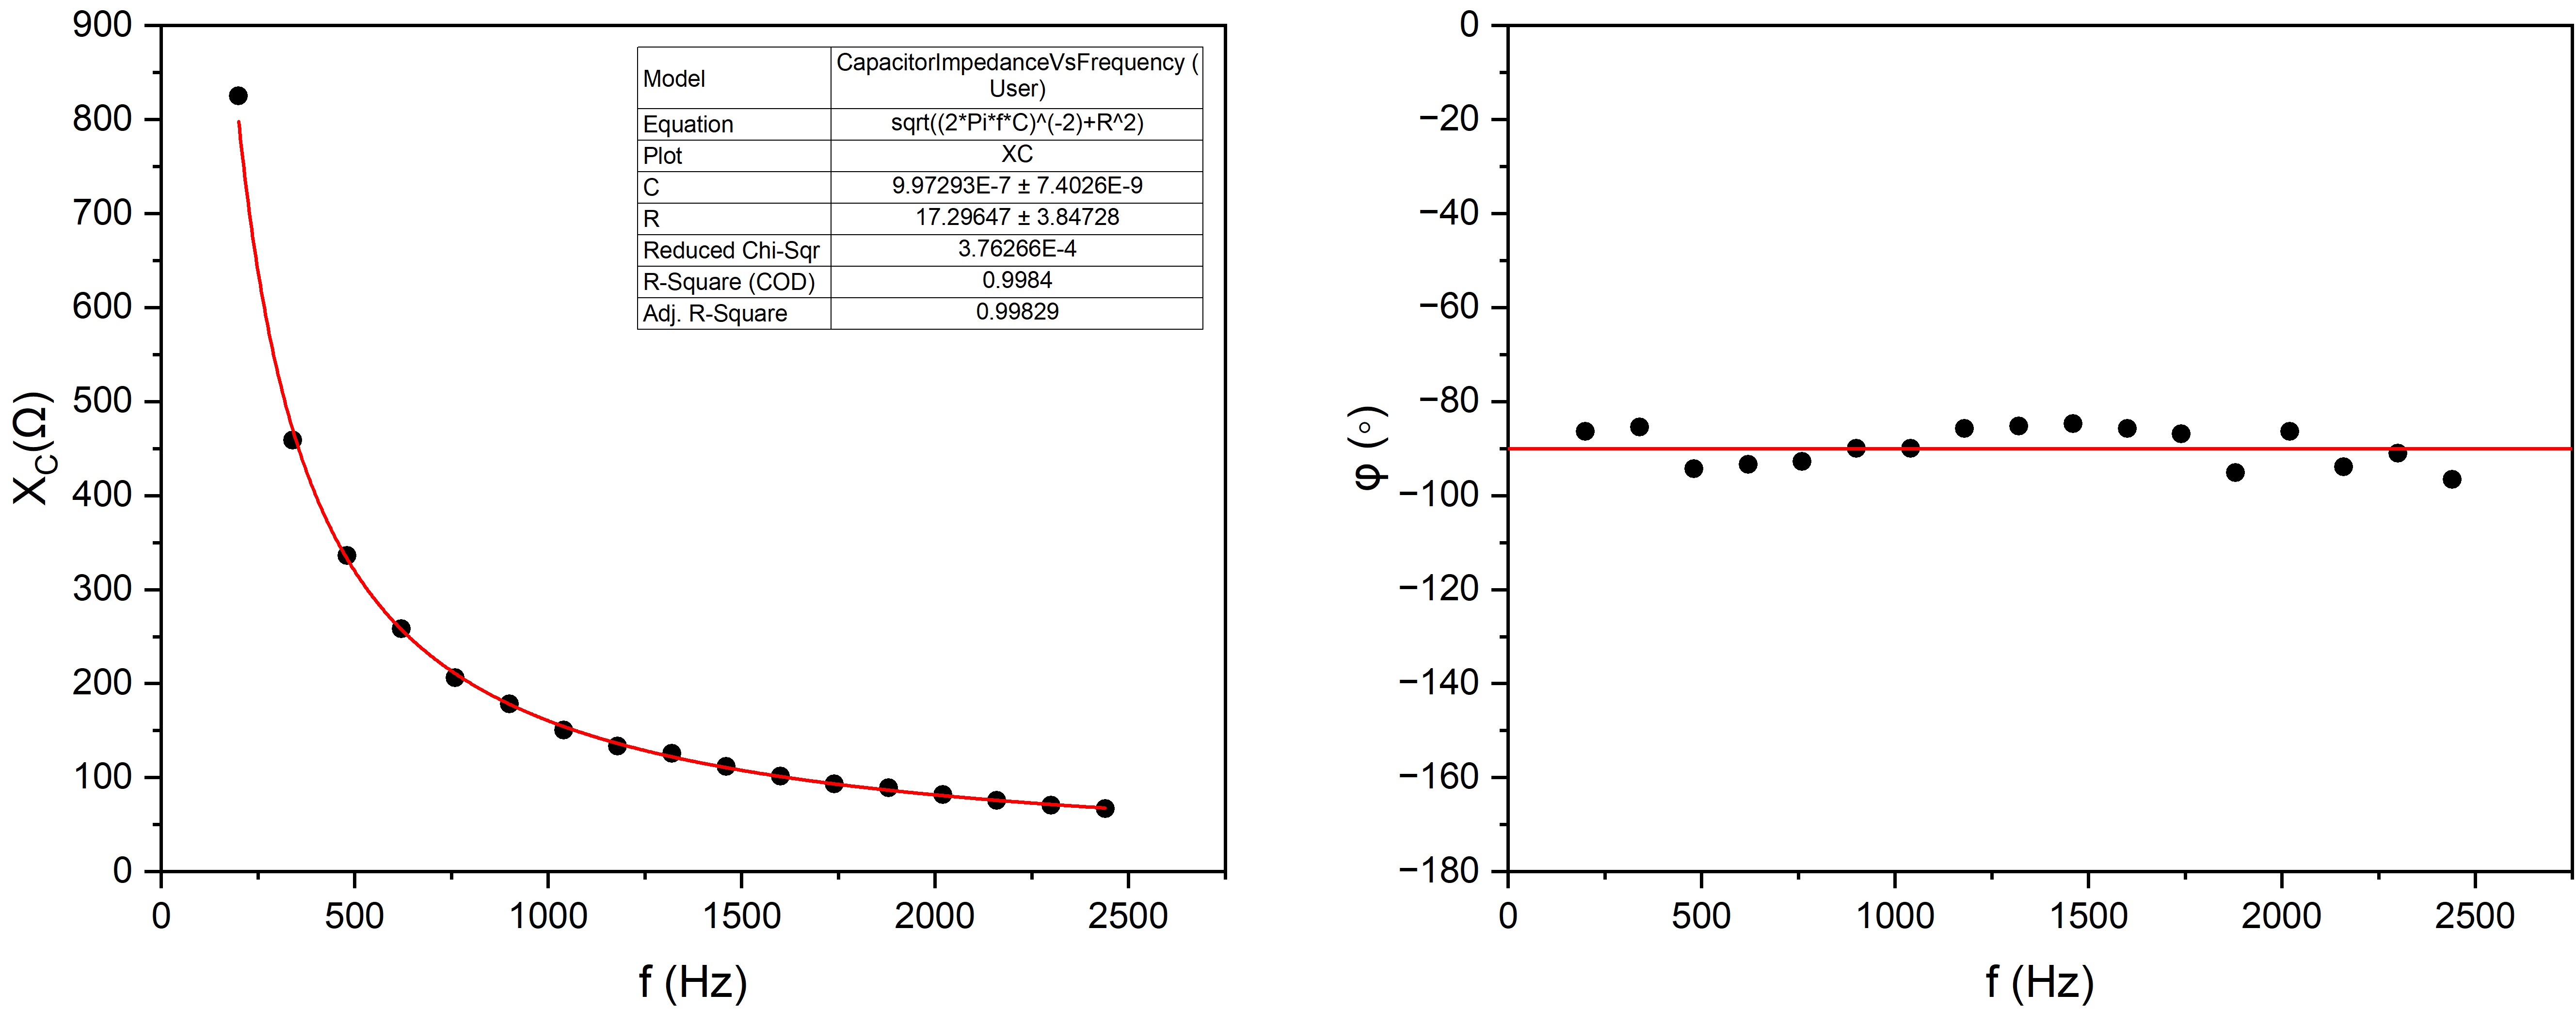
\includegraphics[width=0.9\textwidth]{Capacitor.png}
\end{figure}\par
可以看出实验结果与理论相差无几,并且通过拟合可以得出
\begin{equation*}
    R_\text{L}=\SI{65.0}{\ohm}, R_\text{C}=\SI{17.3}{\ohm}
\end{equation*}
\section{思考题}
\subsection{图 2 中各元件流过的电流如何求得?}
用 $r$ 两端的电流和电压,使用欧姆定律求得。
\subsection{怎样用双踪示波器观察 rL 串联和 rC 串联电路阻抗角的频率特性?}
示波器分别测量 $U_\text{s}$ 和 $U_\text{r}$,同时使用示波器的运算功能得出 $U_\text{L}=U_\text{s}-U_\text{r}$ 的波形,这样就可以通过数格子或者自动测量功能测量出阻抗角。
\section{实验心得}
    本次实验研究了 R、L、C 元件阻抗特性,对于阻抗又有了更加清晰明确的认知,虽然数格子测量阻抗角误差较大,但是实验结果基本符合预期,同时提升了我使用示波器的技能。
\clearpage
\section{原始数据}
原始数据采用 Excel 记录,未在纸上记录,下面给出签名页和 Excel 数据。
\begin{center}
    \framebox{\rotatebox{-90}{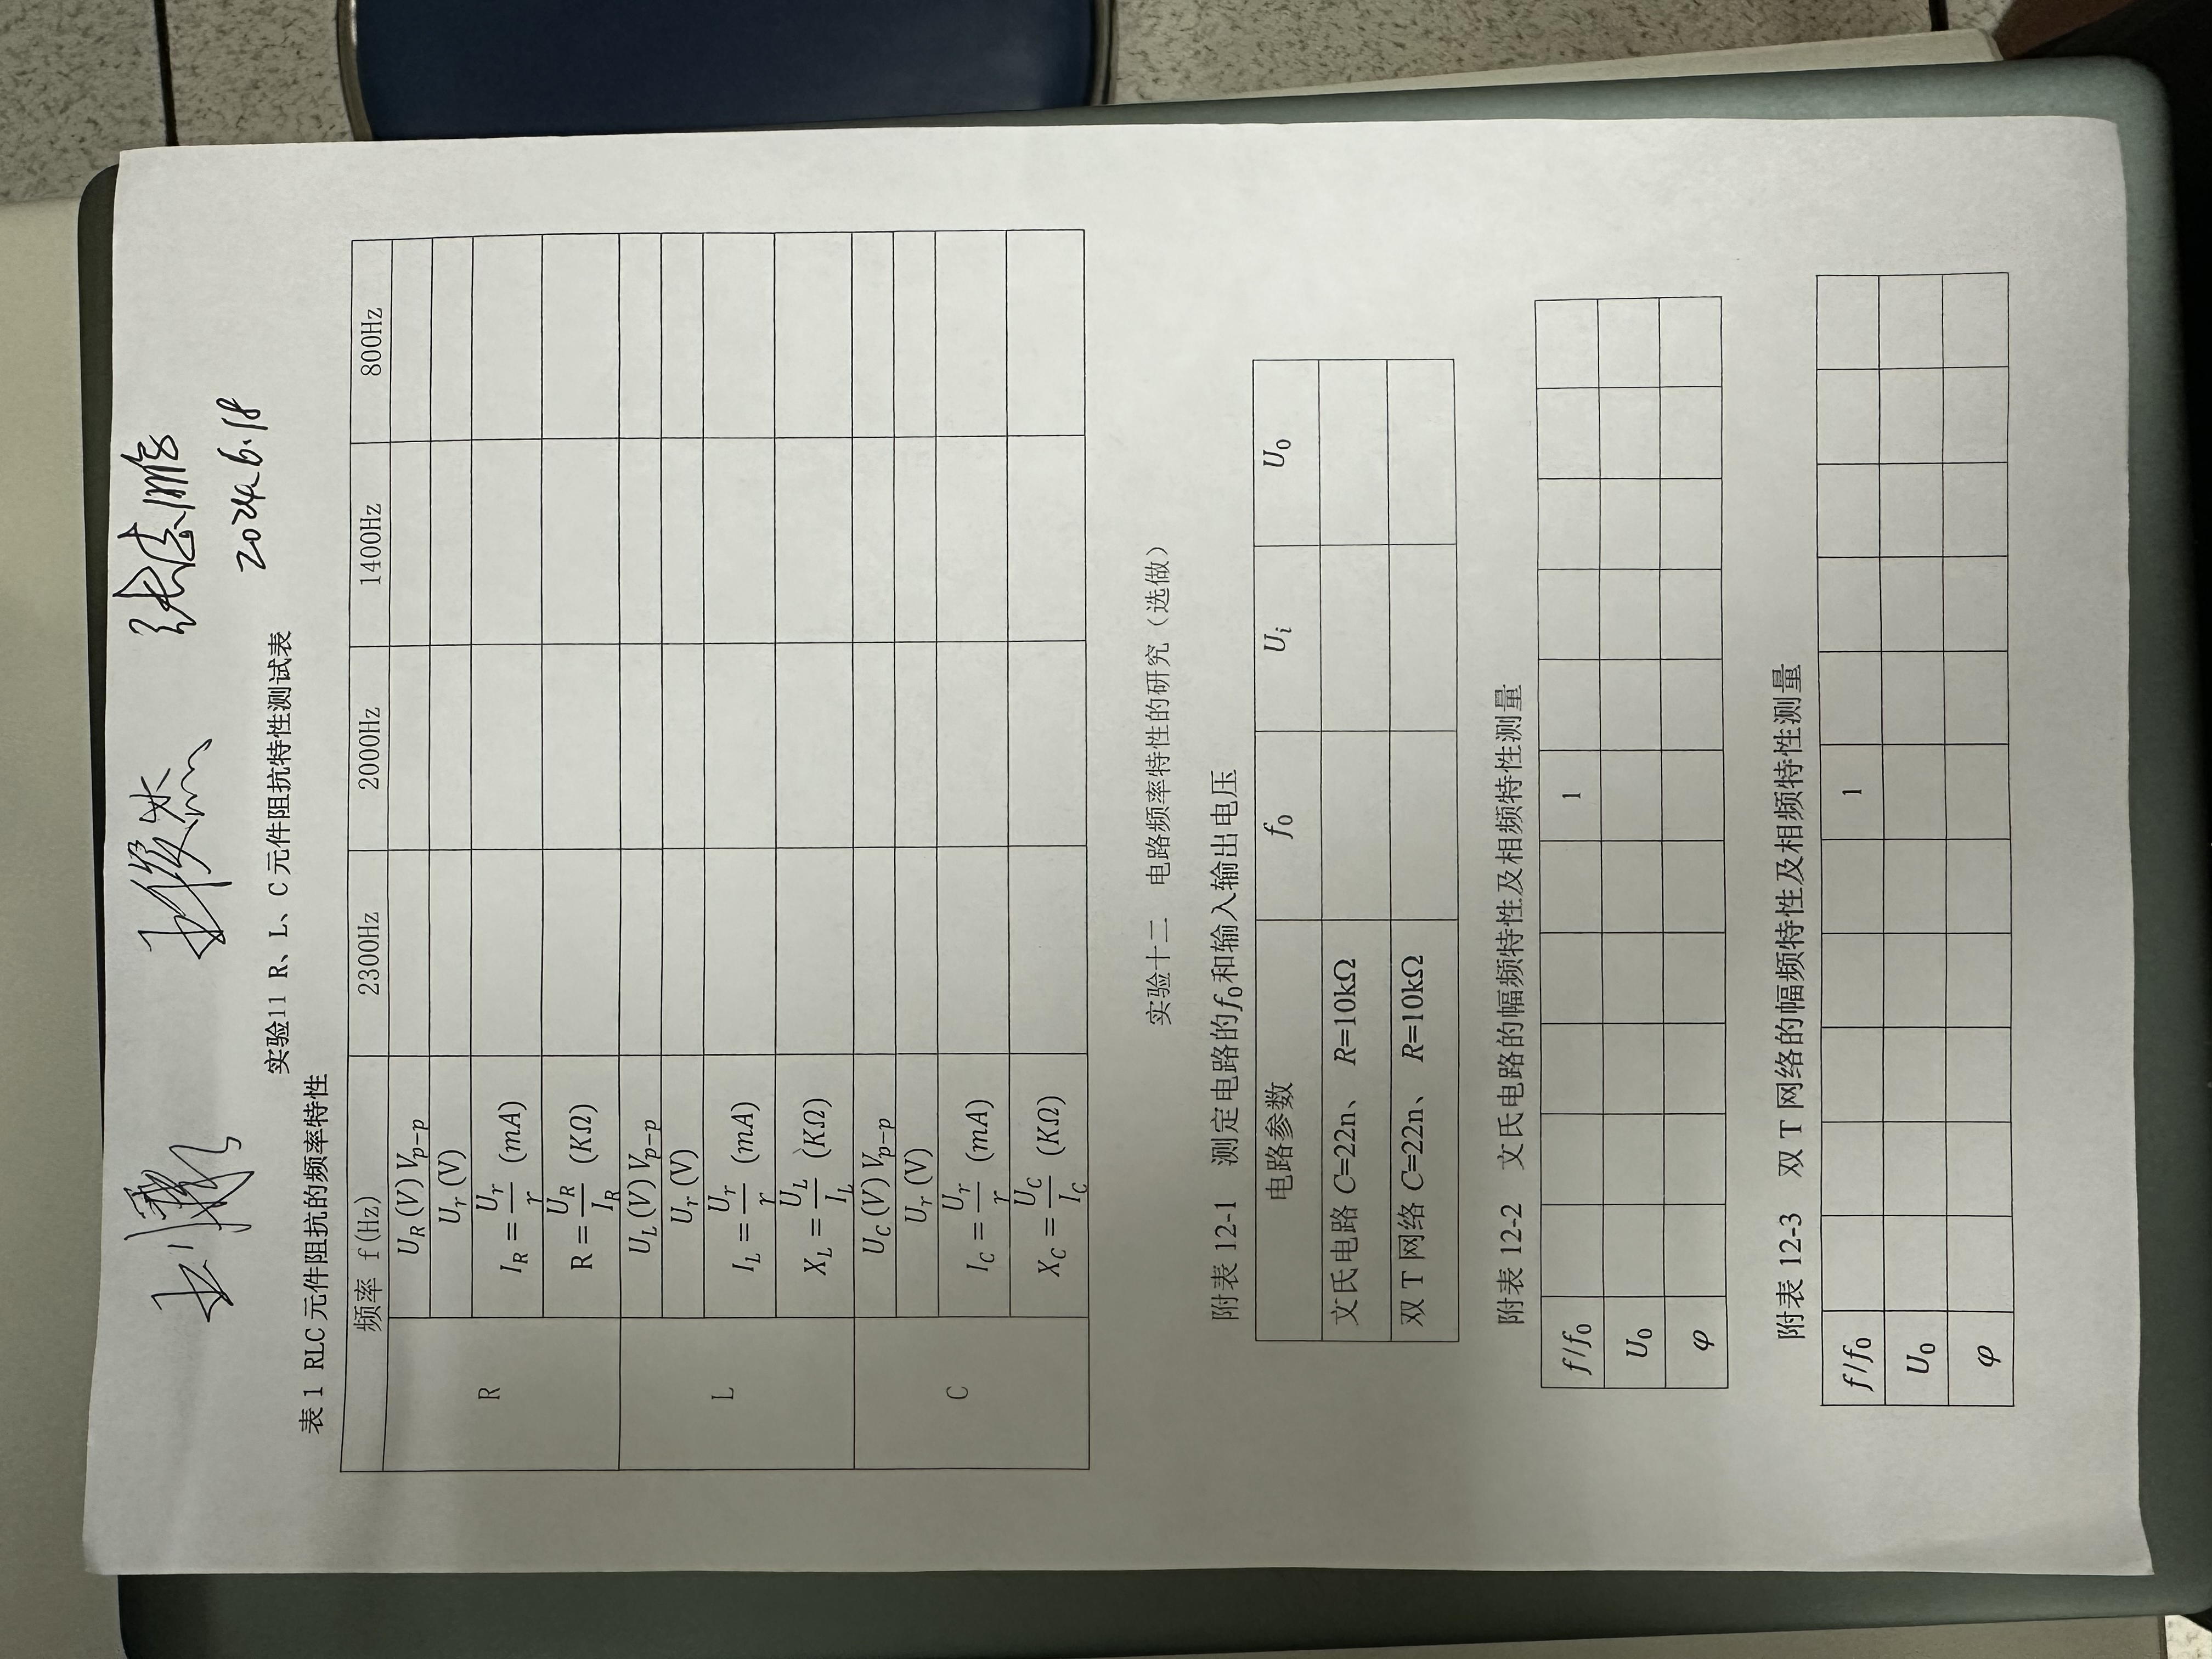
\includegraphics[height=0.8\textwidth]{rawdata.jpg}}}
\end{center}

\begin{center}
    \framebox{\rotatebox{-90}{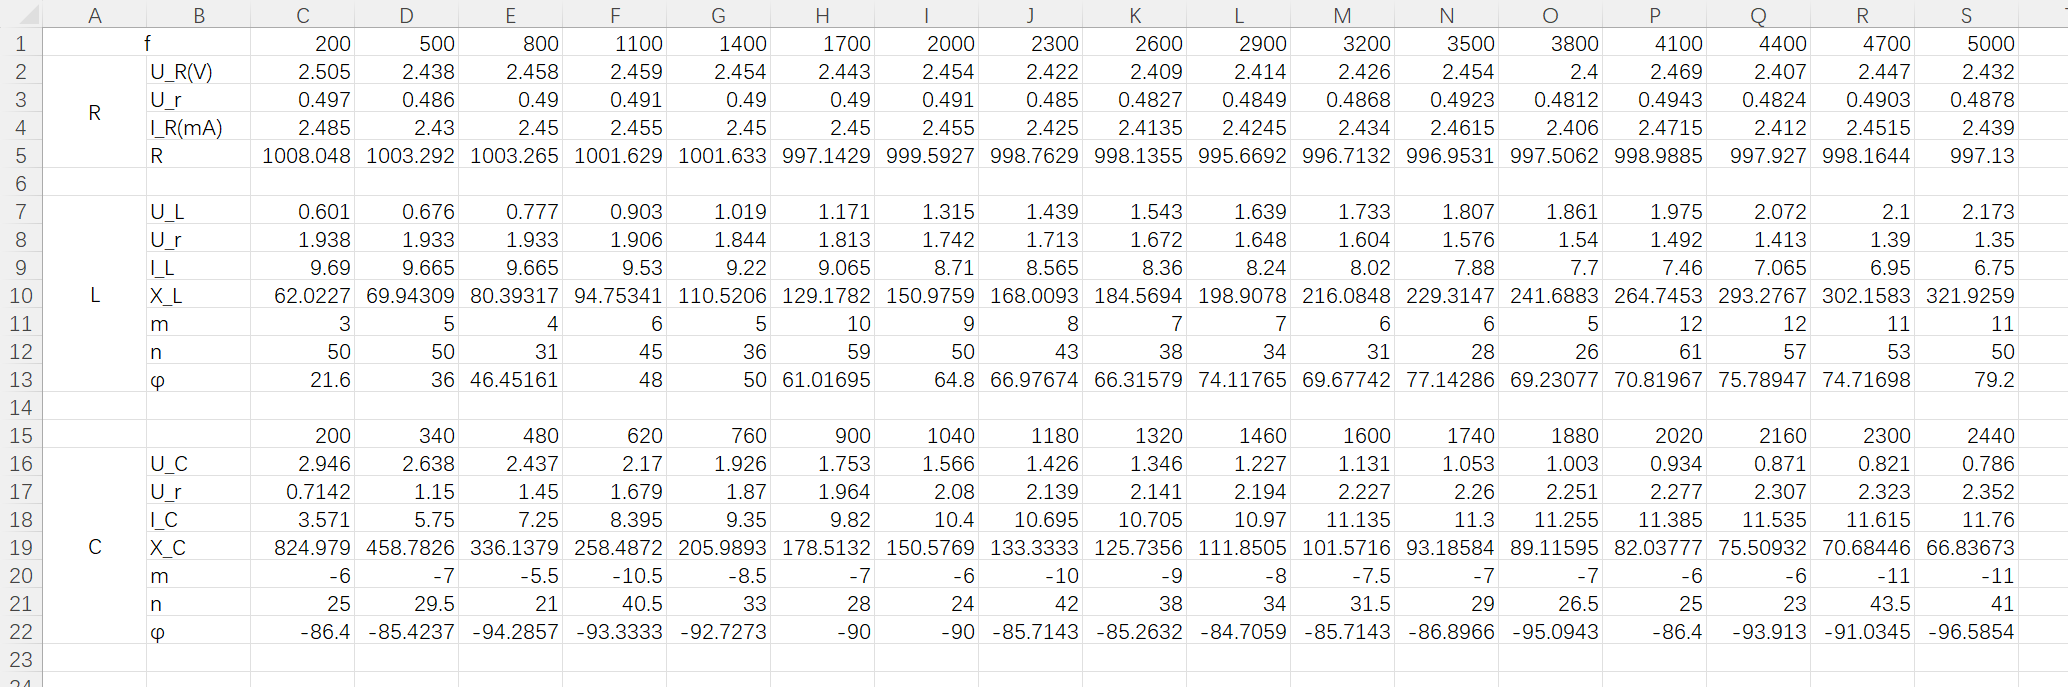
\includegraphics[width=0.95\textheight]{rawdata2.png}}}
\end{center}
\end{document}